% ------------------------------------------------------------------------------
% TYPO3 Version 9.4 - What's New (English Version)
%
% @author	Michael Schams <schams.net>
% @license	Creative Commons BY-NC-SA 3.0
% @link		https://typo3.org/help/documentation/whats-new/
% @language	English
% ------------------------------------------------------------------------------


\section{Introduction}
\begin{frame}[fragile]
	\frametitle{Introduction}

	\begin{center}\huge{Introduction}\end{center}
	\begin{center}\huge{\color{typo3darkgrey}\textbf{The Facts}}\end{center}

\end{frame}

% ------------------------------------------------------------------------------
% TYPO3 Version 9.4 - The Facts

\begin{frame}[fragile]
	\frametitle{Introduction}
	\framesubtitle{TYPO3 Version 9.4 - The Facts}

	\begin{itemize}
		\item Release date: 04 September 2018
		\item Release type: Sprint Release
	\end{itemize}

	\begin{figure}
		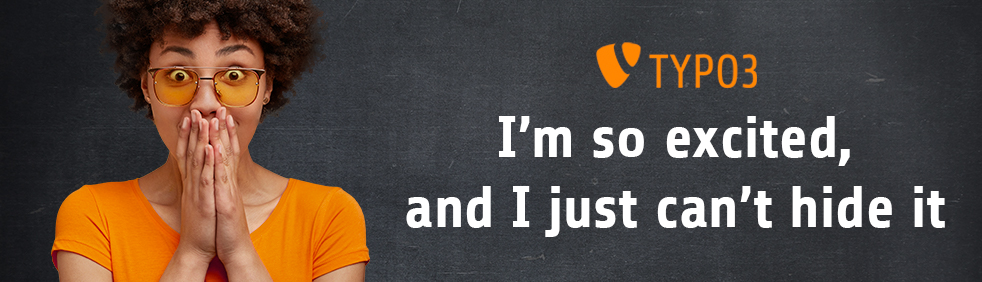
\includegraphics[width=0.95\linewidth]{Introduction/typo3-v94-banner.jpg}
	\end{figure}

\end{frame}

% ------------------------------------------------------------------------------
% System Requirements

\begin{frame}[fragile]
	\frametitle{Introduction}
	\framesubtitle{System Requirements}

	\begin{itemize}
		\item PHP version 7.2 or higher
		\item PHP settings:

			\begin{itemize}
				\item \texttt{memory\_limit} >= 256M
				\item \texttt{max\_execution\_time} >= 240s
				\item \texttt{max\_input\_vars} >= 1500
				\item compilation option \texttt{-}\texttt{-disable-ipv6} must \underline{not} be used
			\end{itemize}

		\item Most database servers supported by \textbf{Doctrine DBAL} also work with TYPO3.
			Tested DB engines are for example:
	\end{itemize}

	\begin{figure}
		
\includegraphics[width=0.80\linewidth]{Introduction/logo-databases.png}
	\end{figure}

\end{frame}

% ------------------------------------------------------------------------------
% Development, Release and Maintenance Timeline

\begin{frame}[fragile]
	\frametitle{Introduction}
	\framesubtitle{Development, Release and Maintenance Timeline}

	\textbf{TYPO3 v9}

	\begin{figure}
		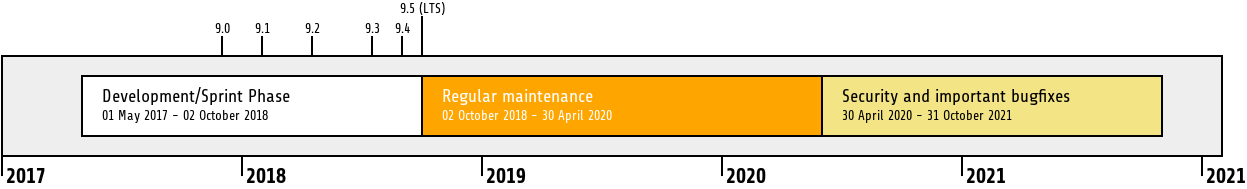
\includegraphics[width=1\linewidth]{Introduction/typo3-v9-lifecycle.png}
	\end{figure}

	\textbf{Extended Support}\newline
	\smaller
		The \href{https://typo3.com}{TYPO3 GmbH} offers further support options
		for TYPO3 v9 LTS even after 31 October 2021 for up to two additional
		years.
	\normalsize

%	\url{https://typo3.com/our-services/extended-support/}

\end{frame}

% ------------------------------------------------------------------------------
% TYPO3 v9 Roadmap

\begin{frame}[fragile]
	\frametitle{Introduction}
	\framesubtitle{TYPO3 v9 Roadmap}

	Release dates and their primary focus:

	\begin{itemize}

		\item v9.0 \tabto{1.1cm}12/Dec/2017\tabto{3.4cm}Install Tool and Page Tree Refactoring,\newline
			\tabto{3.4cm}Unified Page Translations
		\item v9.1 \tabto{1.1cm}30/Jan/2018\tabto{3.4cm}Redirect Handling
		\item v9.2 \tabto{1.1cm}10/Apr/2018\tabto{3.4cm}Site Handling
        \item v9.3 \tabto{1.1cm}12/Jun/2018\tabto{3.4cm}SEO and URL Routing Preparations
		\item
			\begingroup
				\color{typo3orange}
                    v9.4 \tabto{1.1cm}04/Sep/2018\tabto{3.4cm}URL Routing for Pages
			\endgroup
		\item v9.5 \tabto{1.1cm}02/Oct/2018\tabto{3.4cm}LTS Release

	\end{itemize}

	\smaller
		\url{https://typo3.org/article/typo3-v9-roadmap/}\newline
		\url{https://typo3.org/cms/roadmap/}
	\normalsize

\end{frame}

% ------------------------------------------------------------------------------
% Installation

\begin{frame}[fragile]
	\frametitle{Introduction}
	\framesubtitle{Installation}

	\begin{itemize}
		\item Official \textit{classic} installation procedure under Linux/Mac OS X\newline
			(DocumentRoot for example \texttt{/var/www/site/htdocs}):
		\begin{lstlisting}
$ cd /var/www/site
$ wget --content-disposition get.typo3.org/9.4
$ tar xzf typo3_src-9.4.0.tar.gz
$ cd htdocs
$ ln -s ../typo3_src-9.4.0 typo3_src
$ ln -s typo3_src/index.php
$ ln -s typo3_src/typo3
$ touch FIRST_INSTALL
		\end{lstlisting}

		\item Symbolic links under Microsoft Windows:

			\begin{itemize}
				\item Use \texttt{junction} under Windows XP/2000
				\item Use \texttt{mklink} under Windows Vista and Windows 7 and higher
			\end{itemize}

	\end{itemize}
\end{frame}

% ------------------------------------------------------------------------------
% Installation using composer

\begin{frame}[fragile]
	\frametitle{Installation and Upgrade}
	\framesubtitle{Installation Using \texttt{composer}}

	\begin{itemize}
		\item Installation using \textit{composer} under Linux, Mac OS X and Windows 10:

			\begin{lstlisting}
$ cd /var/www/site/
$ composer create-project typo3/cms-base-distribution CmsBaseDistribution ^9
			\end{lstlisting}

		\item Alternatively, create your custom \texttt{composer.json} file and run:

			\begin{lstlisting}
$ composer install
			\end{lstlisting}

			Further details and examples for \texttt{composer.json} files are available at:\newline
			\smaller
				\href{https://composer.typo3.org}{https://composer.typo3.org}
			\normalsize

	\end{itemize}
\end{frame}

% ------------------------------------------------------------------------------
